
%%%%%%%%%%%%%%%%%%%%%%% file typeinst.tex %%%%%%%%%%%%%%%%%%%%%%%%%
%
% Author: Mauricio Matamoros
% Updated: July 3, 2017
% Contact: mauricio@robocupathome.org
%
% This is the LaTeX source for the TDPTemplate using
% the LaTeX document class 'llncs.cls' Springer LNAI format
% used in the RoboCup Symposium submissions.
% http://www.springer.com/computer/lncs?SGWID=0-164-6-793341-0
%
% It may be used as a template for your own TDP - copy it
% to a new file with a new name and use it as the basis
% for your Team Description Paper
%
% NB: the document class 'llncs' has its own and detailed documentation, see
% ftp://ftp.springer.de/data/pubftp/pub/tex/latex/llncs/latex2e/llncsdoc.pdf
%
% Remark: Last page with specs won't be included in Camera ready TDP's.
%
%%%%%%%%%%%%%%%%%%%%%%%%%%%%%%%%%%%%%%%%%%%%%%%%%%%%%%%%%%%%%%%%%%%

\documentclass[runningheads,a4paper]{llncs}
\usepackage{amssymb}
\setcounter{tocdepth}{3}
\usepackage{graphicx}
\usepackage{amssymb}
\usepackage[utf8]{inputenc}
\usepackage[hidelinks]{hyperref}
\usepackage{url}
\usepackage{float}
\usepackage{amsmath}
\usepackage{graphicx}
\usepackage{wrapfig}
\usepackage{fancyhdr}
\usepackage{titling}
\usepackage{xcolor}
\usepackage{lipsum}
\usepackage{ragged2e}
\input{macros}



\makeatletter
\DeclareRobustCommand{\textsupsub}[2]{{%
  \m@th\ensuremath{%
    ^{\mbox{\fontsize\sf@size\z@#1}}%
    _{\mbox{\fontsize\sf@size\z@#2}}%
  }%
}}
\makeatother

%%%%%%%%%%%%%%%%%%%%%%%%%%%%%%%%%%%%%%%%%%%%%%%%%%%%%%%%%%%%%%%%%%%%%%%%%%%%%%%%%%%%
%
% Title
%
%%%%%%%%%%%%%%%%%%%%%%%%%%%%%%%%%%%%%%%%%%%%%%%%%%%%%%%%%%%%%%%%%%%%%%%%%%%%%%%%%%%%
\title{Immortals 2019 Extended Team Description Paper}

\author{\normalsize Omid Najafi Koopai{\textsupsub{\small\texttt{1}}{}}, 
MohammadAli Ghasemieh{\textsupsub{\small\texttt{2}}{}}, 
Mehran Khanloghi{\textsupsub{\small\texttt{3}}{}}, \\
\normalsize AliReza Mohammadi{\textsupsub{\small\texttt{3}}{}}, 
AmirMahdi Matin{\textsupsub{\small\texttt{3}}{}},
AmirMahdi Torabian{\textsupsub{\small\texttt{4}}{}}
}
\institute{Sharif University of Technology, \\
\texttt{http://devoted-web-site.url}}


\begin{document}
\maketitle

\center{
\texttt{\small 1} Sharif University of Technology\\
\texttt{\small 2} Pars University of Art\\
\texttt{\small 3} University of Tehran\\
\texttt{\small 4} University of Science and Technology\\
\texttt{http://www.immortals-robotics.com}
}

%%%%%%%%%%%%%%%%%%%%%%%%%%%%%%%%%%%%%%%%%%%%%%%%%%%%%%%%%%%%%%%%%%%%%%%%%%%%%%%%%%%%
%
% Abstract
%
%%%%%%%%%%%%%%%%%%%%%%%%%%%%%%%%%%%%%%%%%%%%%%%%%%%%%%%%%%%%%%%%%%%%%%%%%%%%%%%%%%%%

\begin{abstract}
This paper describes the recent works done by the Immortals team, a team consisting of undergraduate engineering students, currently focusing on the Small Size League. There were changes applied to the mechanics and electronics of the robots in the previuos year. This year, the team focused on solving the issues which were observed during the recent competitions including RoboCup 2018, Montréal. The goal is to reach to a reliable design where there is no need for any robot substitution due to damages during a match. In addition to the current robot, there is a 3D printed robot which was introduced in the previous year by this team and has been improved and tested in the recent competitions.
%In your abstract, please state your main research line and your achievements of this year (on which problem or set of problems are you focusing all the team efforts). Tell why this research is important, how are you approaching to the problem solution and which results do you expect to obtain.

\end{abstract}


%%%%%%%%%%%%%%%%%%%%%%%%%%%%%%%%%%%%%%%%%%%%%%%%%%%%%%%%%%%%%%%%%%%%%%%%%%%%%%%%%%%%
\justify
\section{Introduction}
The Immortals Robotics Team is a team of undergraduate students from Sharif, Tehran and Pars University. The team started the Small Size League (SSL) project in the summer of 2007 and produced its first robot after one year, there have been major revisions made in the designs of the robots since then. In this paper the most recent changes on the designs and achivments made by the team will be shared with the reader whom, wants to design or modify an SSL robot. There is also a new type of robot which was introduced by this team in the past year known as the 3D-Printed robot [1,4].
\begin{figure}
	\centering
	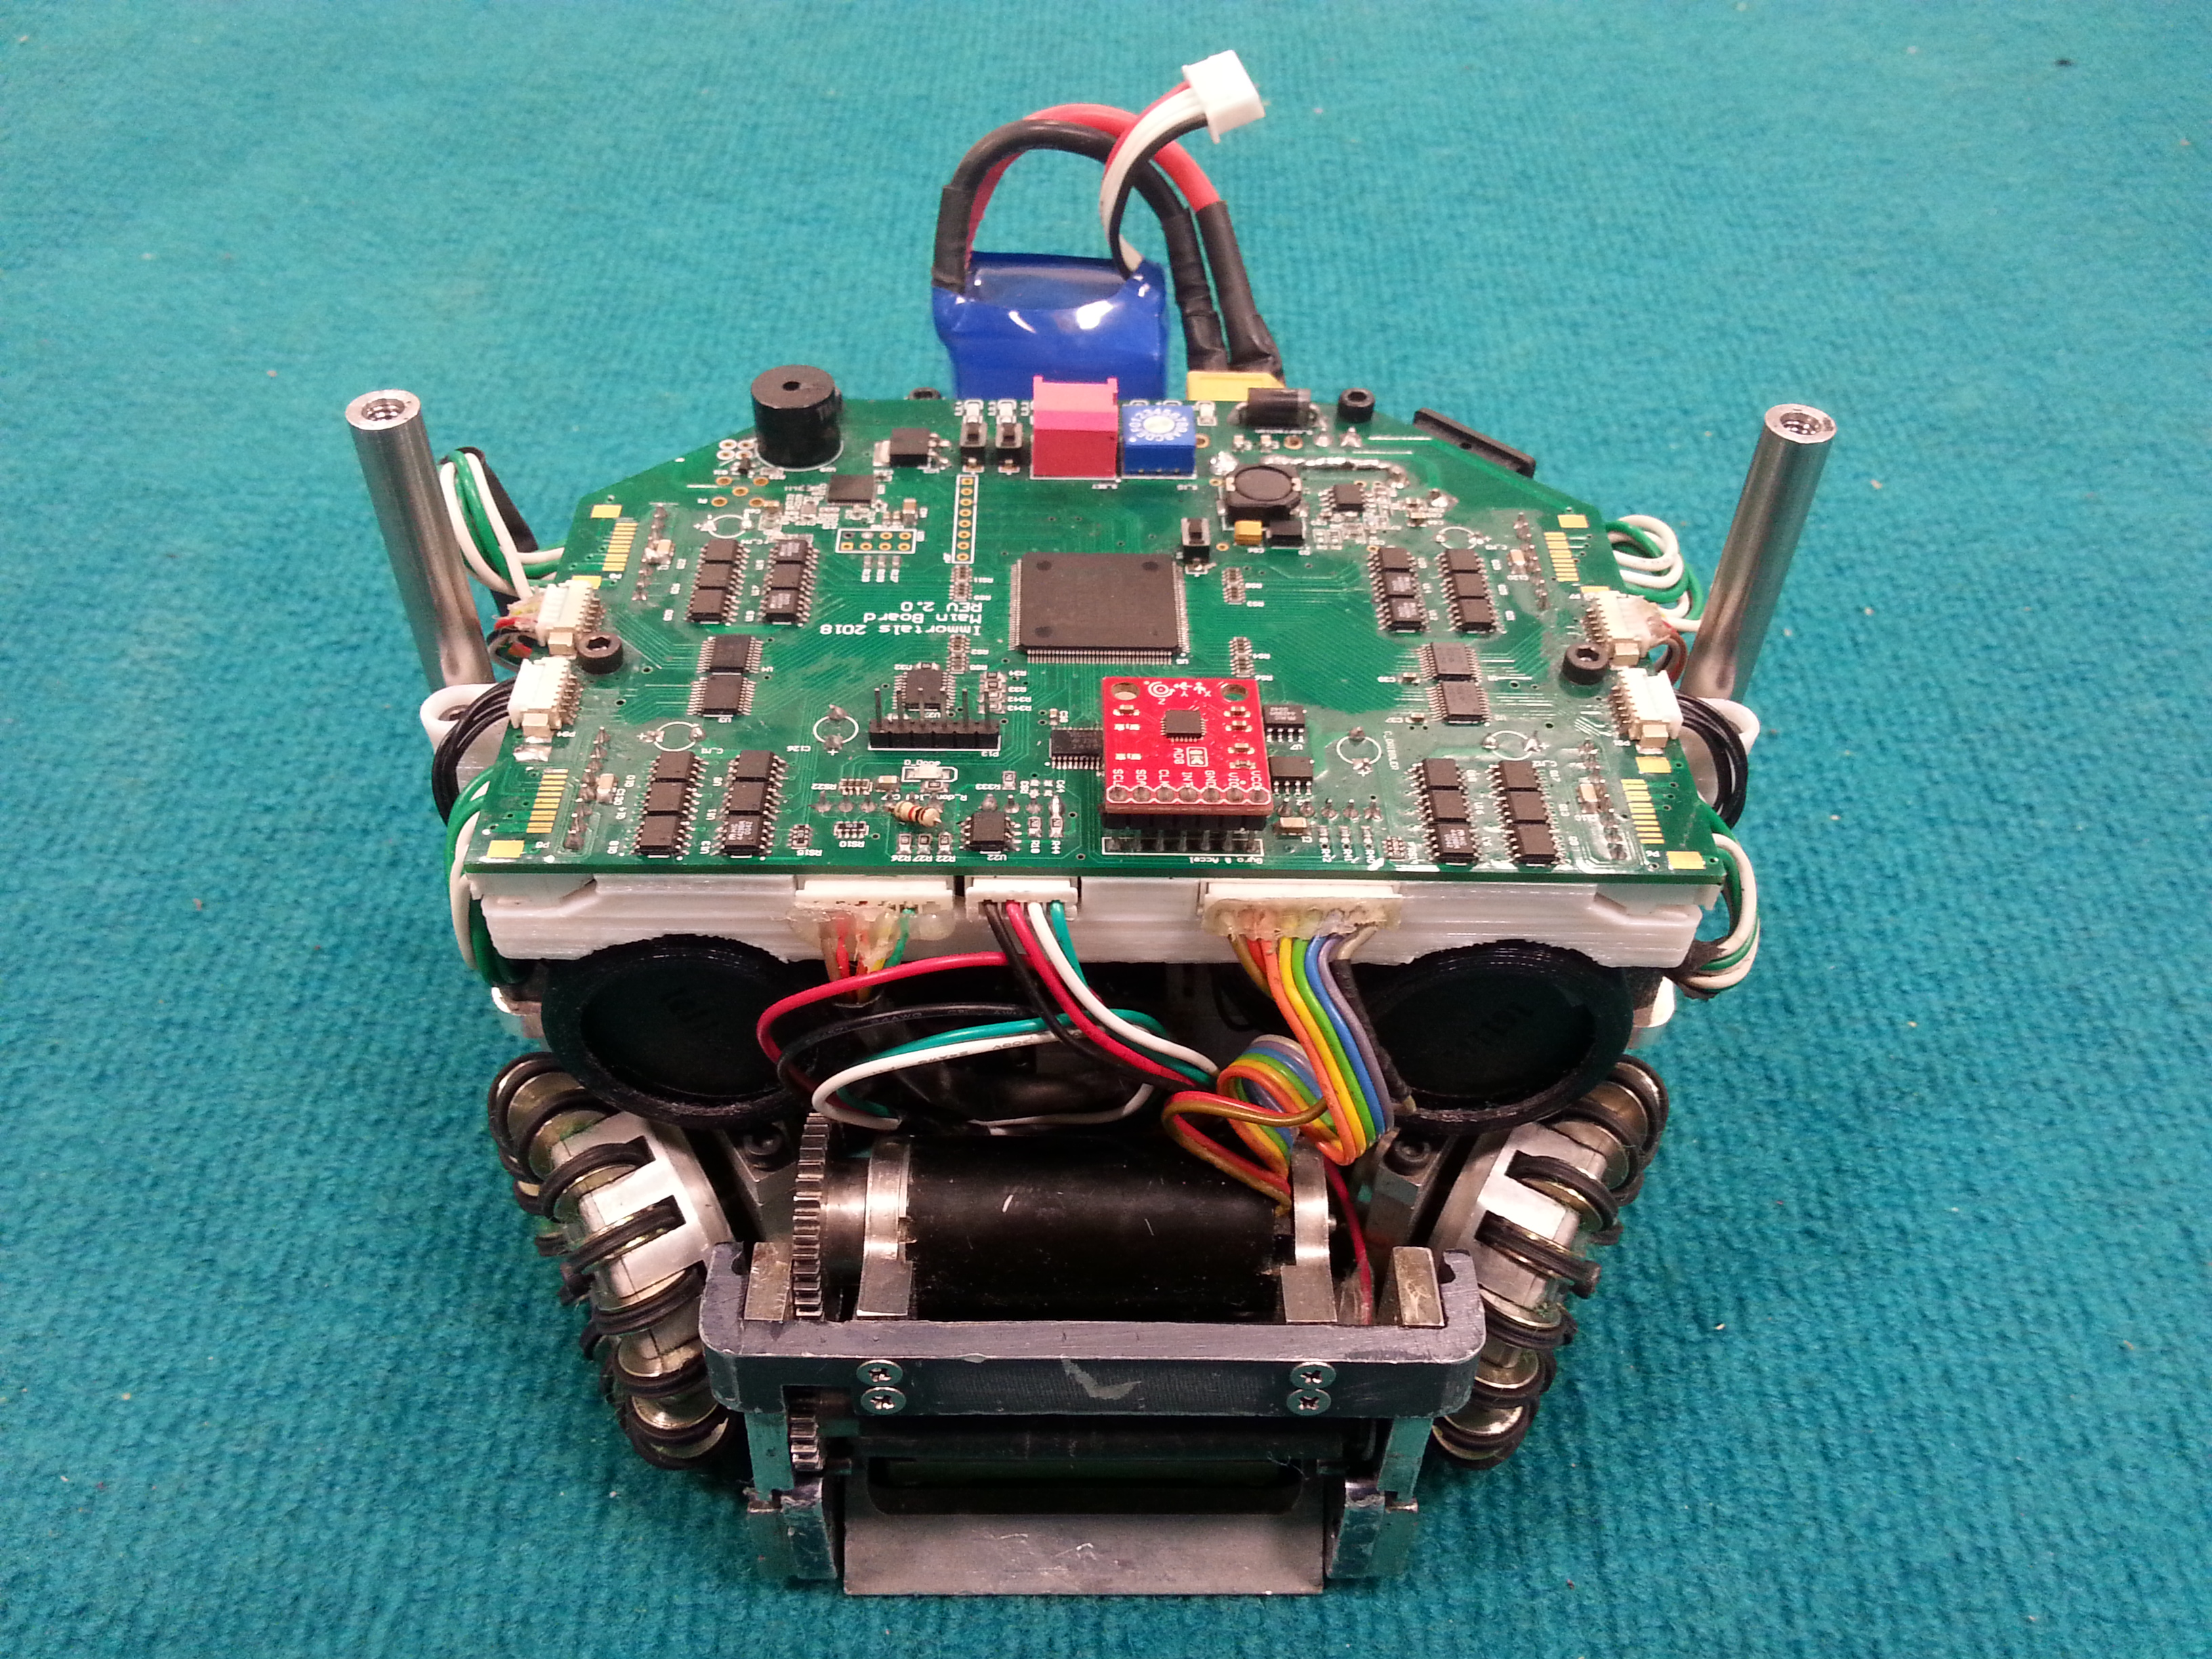
\includegraphics[width=0.8\textwidth]{images/CURRENT.jpg}
	\caption{Current Immortals Robot}
	\label{fig:CURRENT_ROBOT}
\end{figure}

%\section{TDP contents}
%While writing the TDP, focus on your current research, clearly stating all scientific contribution, and why are they important for you and the league. The length of the TDP is limited to 8 pages including references. Exceeding the number of pages will automatically void your application.
%
%Although reviewers share a common background in the domain of service robotics, is very unlikely that they are actively involved in your research field. The organizing committee kindly asks authors to keep this in mind and write in a more descriptive and less analytic way. The main goal of a TDP is tell others about your latest practical achievement, how your team managed to solve the problem, what strategy was chosen and why, while at the same time trying to convince your reader that what you are doing is useful or applicable in a daily life scenario.
%
%The Team Description Paper shall use the \textit{Springer LNAI format}\footnotemark used in the RoboCup Symposium submissions, and has a hard limit of 8 pages without altering margins or spacing (including references but excluding the annex). Please notice that changes to the margins, space between paragraphs, and font size are not allowed (such TDP will be rejected). We suggest to leave the hardware and software description for the end of the paper in the annex.\footnotetext{\url{http://www.springer.com/computer/lncs?SGWID=0-164-6-793341-0}}
%
%\textbf{Important Notice:} Attaching to the requested format is important for the camera ready version of the TDPs can be included in the memories of the competition.
%
%Remember that the TDP must contain the following information:
%
%\begin{itemize}
%	\item Innovative technology and scientific contribution
%	\item Focus of research/research interests
%	\item Re-usability of the system for other research groups
%	\item Applicability of the robot in the real world
%	\item \textbf{DSPL \& SSPL:} When the robot depicted in the TDP or Team Video is different from the league's standard one, the TDP must clearly state how the addressed approach and described software will be adapted to the standard platform robot.
%\end{itemize}
%
%\textbf{Remark:} The language for the TDP body, its graphics, tables, images, and all additional content must be English. Content in other languages must be translated.
%
%\subsection{TDP Annex}
%The TDP's Robot Description Annex is an appendix of arbitrary length that should be attached at the end of the TDP and summarizes the robot's software and hardware technical specifications.
%
%When present, the annex must contain the following information:
%
%\begin{itemize}
%	\item Photo(s) of the robot
%	\item \textbf{OPL only:} Brief, compact description of the robot's hardware.
%	\item \textbf{DSPL \& SSPL:} Please skip hardware description.
%	\item Brief, compact description of the robot's software (including commercial products, freeware, Open Source, etc.).
%	\item List of all external computing devices and the software running on them.
%	\item List of all cloud computing resources intended to be used.
%	\item Brief, compact description of all external devices (e.g. smart home devices, transceivers, helper robots, etc.).
%\end{itemize}
%
%Examples are provided at the end of this document in
%\hyperlink{page.9}{page~9~(DSPL)},
%\hyperlink{page.10}{page~10~(OPL)}, and
%\hyperlink{page.11}{page~11~(SSPL)}.
%
%\textbf{Copyright note:} All TDPs sent for qualification may be made publicly available in the RoboCup @Home Wiki for further reference. On submitting, teams implicitly grant permission to RoboCup @Home and the RoboCup Federation to copy, distribute, upload, publish, and use the manuscript to promote the event and the league at convenience.
%
%\section{Background}
%% We are Buy n Large. We have no competitors so no background is required.
%\lipsum[1-3]
%
%\section{BnL Trash Seeker Algorithm (Main research)}
%\lipsum[4-10]
%
%\section{BnL All-purpose Speech Recognizer (Main research)}
%\lipsum[11-13]
%
%\section{Other relevant contributions}
%\lipsum[14]
%\subsection{Dirt Detector Algorithm}
%\lipsum[15-17]
%\subsection{Green Plant Seeker Algorithm}
%\lipsum[18-20]
%\subsection{Trash Seeker Algorithm}
%\lipsum[20-22]
%
%\section{Experiments and results}
%\lipsum[23-24]
%
%\section{Conclusions and future work}
%\lipsum[25-26]


%%%%%%%%%%%%%%%%%%%%%%%%%%%%%%%%%%%%%%%%%%%%%%%%%%%%%%%%%%%%%%%%%%%%%%%%%%%%%%%%%%%%
%
% Robot Specifications
%
%%%%%%%%%%%%%%%%%%%%%%%%%%%%%%%%%%%%%%%%%%%%%%%%%%%%%%%%%%%%%%%%%%%%%%%%%%%%%%%%%%%%

%\robospecs
%\newpage
\section{Mechanics}
% In this section briefly describe the software and hardware of the robot
\setlength\intextsep{0pt}
In the past two years there were multiple changes applied to the chip kicker in order to reach the most efficient design. A great number of simulation tests were done on every chip design and after a successful test, the parts were manufactured for real world testing procedures.

\subsection{Chip kickers new design}
Chip kicker is a part which should have a high resistance against impacts, It has to be efficient in transmitting the force applied to it from the chip kicker plunger to the ball. The first improvement in the chip kicker is that $\theta$ (angle between a line which passes through the chip kickers axis of rotation and impact point and the direction of the force vector)has been increased to 90 degrees. With this improvement the force applied to the chip kicker will be completely in the direction of the angular acceleration of the chip kicker. According to the torque relation, It is shown that when the angle between the force and the distance vector turn into 90 degrees, The ball would receive the most impact from that force.\\
\indent The other improvement is to increase the moment of inertia around the chip kickers axis of rotation. This way, more angular acceleration can be achieved by the chip kicker.\\
\indent In this section we will derive a function for angular acceleration of the chip kicker. As known, the relation between the moment of inertia around the chip kickers axis of rotation and sum of torque applied to the chip kicker can be written as:
\begin{equation}
\sum T=I\alpha
\end{equation}
\begin{equation}
T=Fb
\end{equation}
Where b is the vertical distance between the center of the chip kickers pin and the point which force is applied.\\
It is not necessary to calculate the impact force accurately thus, it is assumed that the force applied, is constant to reduce the parameters involved in the new chip kickers design. the impact force is approximated by the equation below:
\begin{equation}
F=\dfrac{m\limits_{plunger} {V}^2\limits_{f-plunger}}{2d}
\end{equation}
Where $m\limits_{plunger}$ is the mass of the plunger and ${V}\limits_{f-plunger}$ is the velocity of plunger exactly before the impact and $d$ is the distance in which the plunger and the chip kicker are in contact during the impact.\\
\indent Below is an expression for the angular acceleration, resulted from the previous equations:
\begin{equation}
\alpha = \dfrac{b m\limits_{plunger} {V}^2\limits_{f-plunger}}{2Id}
\end{equation}
By assuming F as constant, The angular acceleration will be a function of:
\begin{equation}
\alpha=f(\dfrac{b}{I})
\end{equation}
As a result, if the moment of inertia around the axis of rotation reduces by decreasing the mass of the chip kicker or reducing the distance between its center of mass and the axis of rotation, $\alpha$ will increase.
As shown in Fig.\ref{fig:CHIP_SIDE_VIEW}, $\dfrac{b}{I}$ is calculated for both old and new designs:\\
\begin{figure}
	\centering
	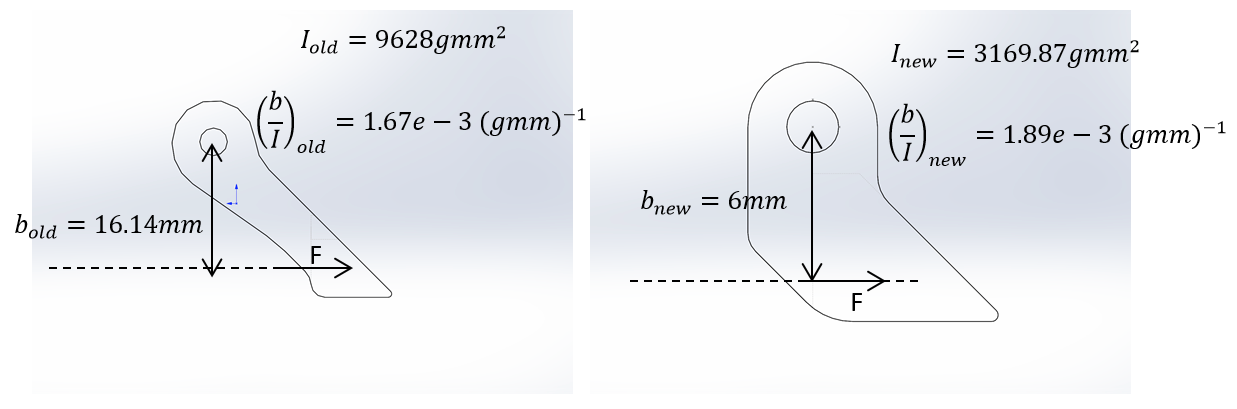
\includegraphics[width=1.0\textwidth]{images/SIDE_VIEW_CHIP.png}
	\caption{$\dfrac{b}{I}$ for old (left) and new (right) design}
	\label{fig:CHIP_SIDE_VIEW}
\end{figure}\\
The results show that $\dfrac{b}{I}$ for the new design is larger than the old one; Therefore, the angular acceleration for the new design should be more than the angular acceleration in the old design. As discussed above, the new design of the chip kicker is much more simple to manufacture ,more reliable and lighter than the old design. %Including these improvements, it also has higher angular acceleration which means reducing its weight won’t affect its functionality.\\
\\
\indent In order to test these results, the impact for both old and new designs were simulated in solid works (as shown in Fig.\ref{fig:SIM2CHIP}).\\
\begin{figure}
	\centering
	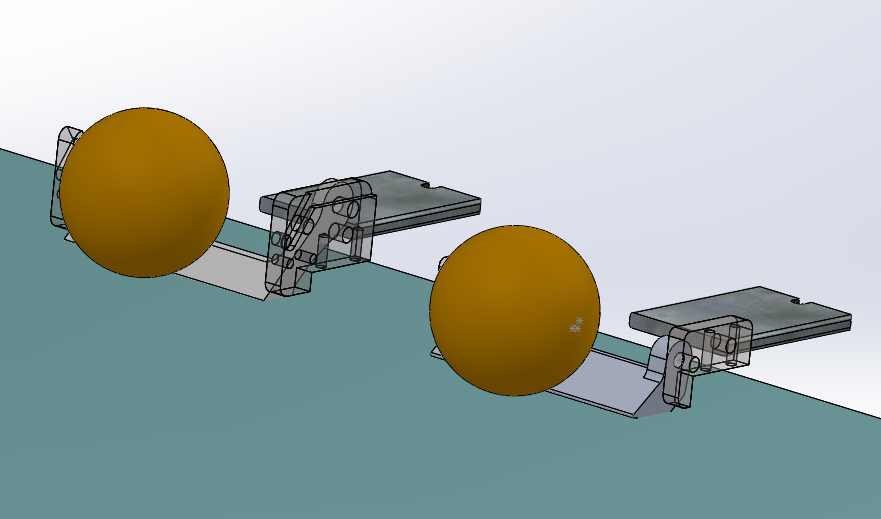
\includegraphics[width=0.8\textwidth]{images/SIM_CHIPx2.png}
	\caption{A view of the old (top left)and new (bottom right)chip kickers in a simulation enviroment}
	\label{fig:SIM2CHIP}
\end{figure}\\
\\
The new chip kicker was tested in a standard SSL field. The results can be seen and compared in Fig. \ref{fig:NEWOLDPLOTBALL}.\\
\begin{figure}
	\centering
	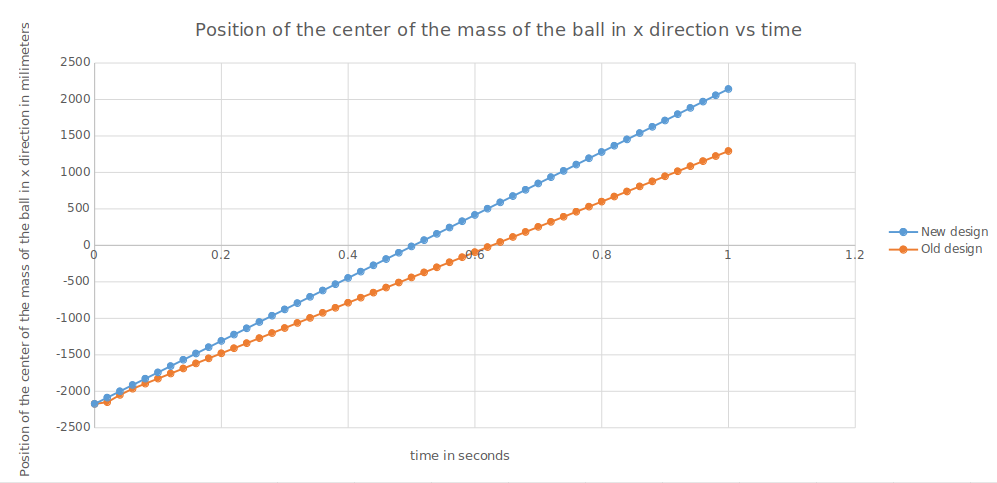
\includegraphics[width=0.8\textwidth]{images/CHIP_POS_PLOT.png}
	\caption{Position time graph for a ball being kicked by the new chip kicker (Blue)and old chip kick(Orange)}
	\label{fig:NEWOLDPLOTBALL}
\end{figure}
%\begin{figure}
%	\centering
%	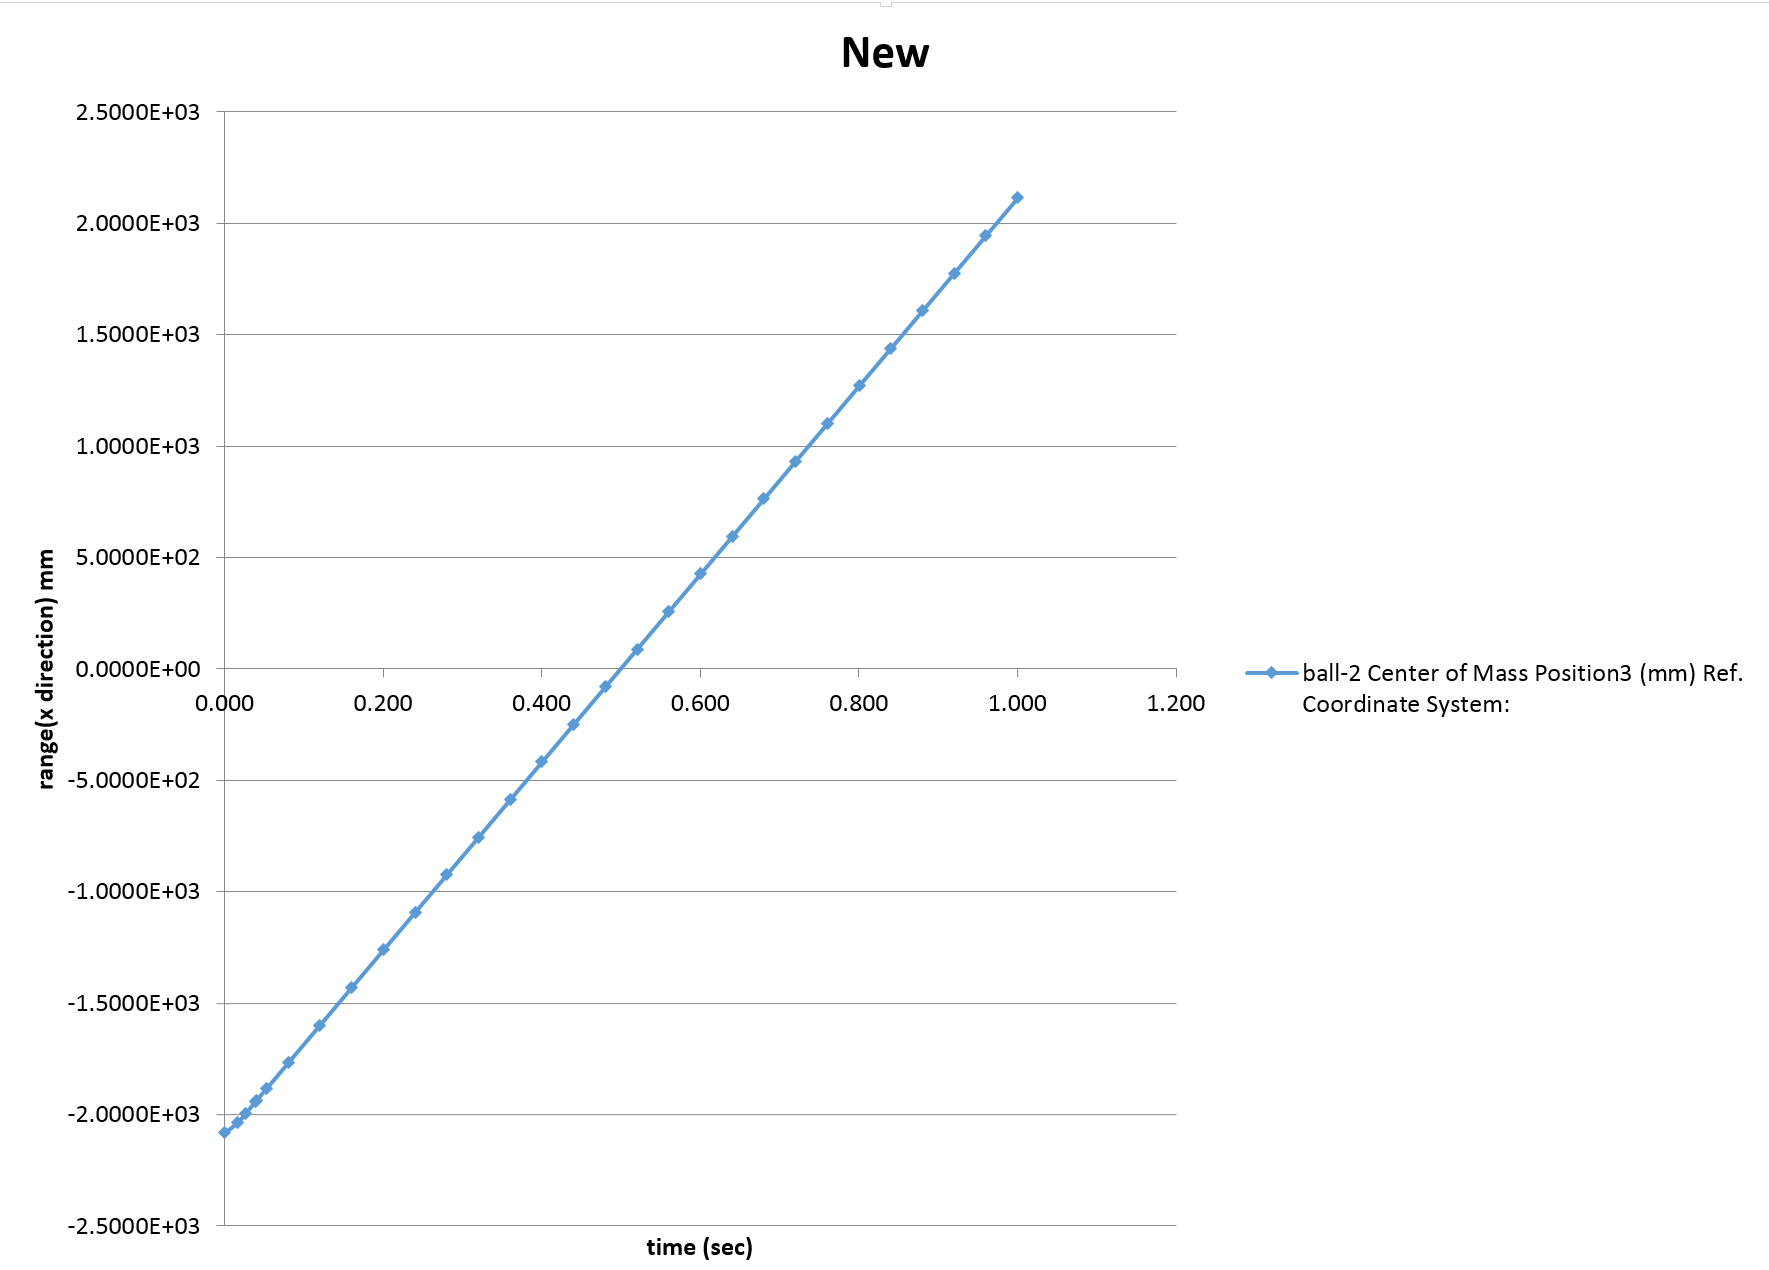
\includegraphics[width=0.8\textwidth]{images/NewBallPlot.png}
%	\caption{Position time graph for a ball being kicked by the new chip kicker}
%	\label{fig:NEWPLOTBALL}
%\end{figure}\\
%\begin{figure}
%	\centering
%	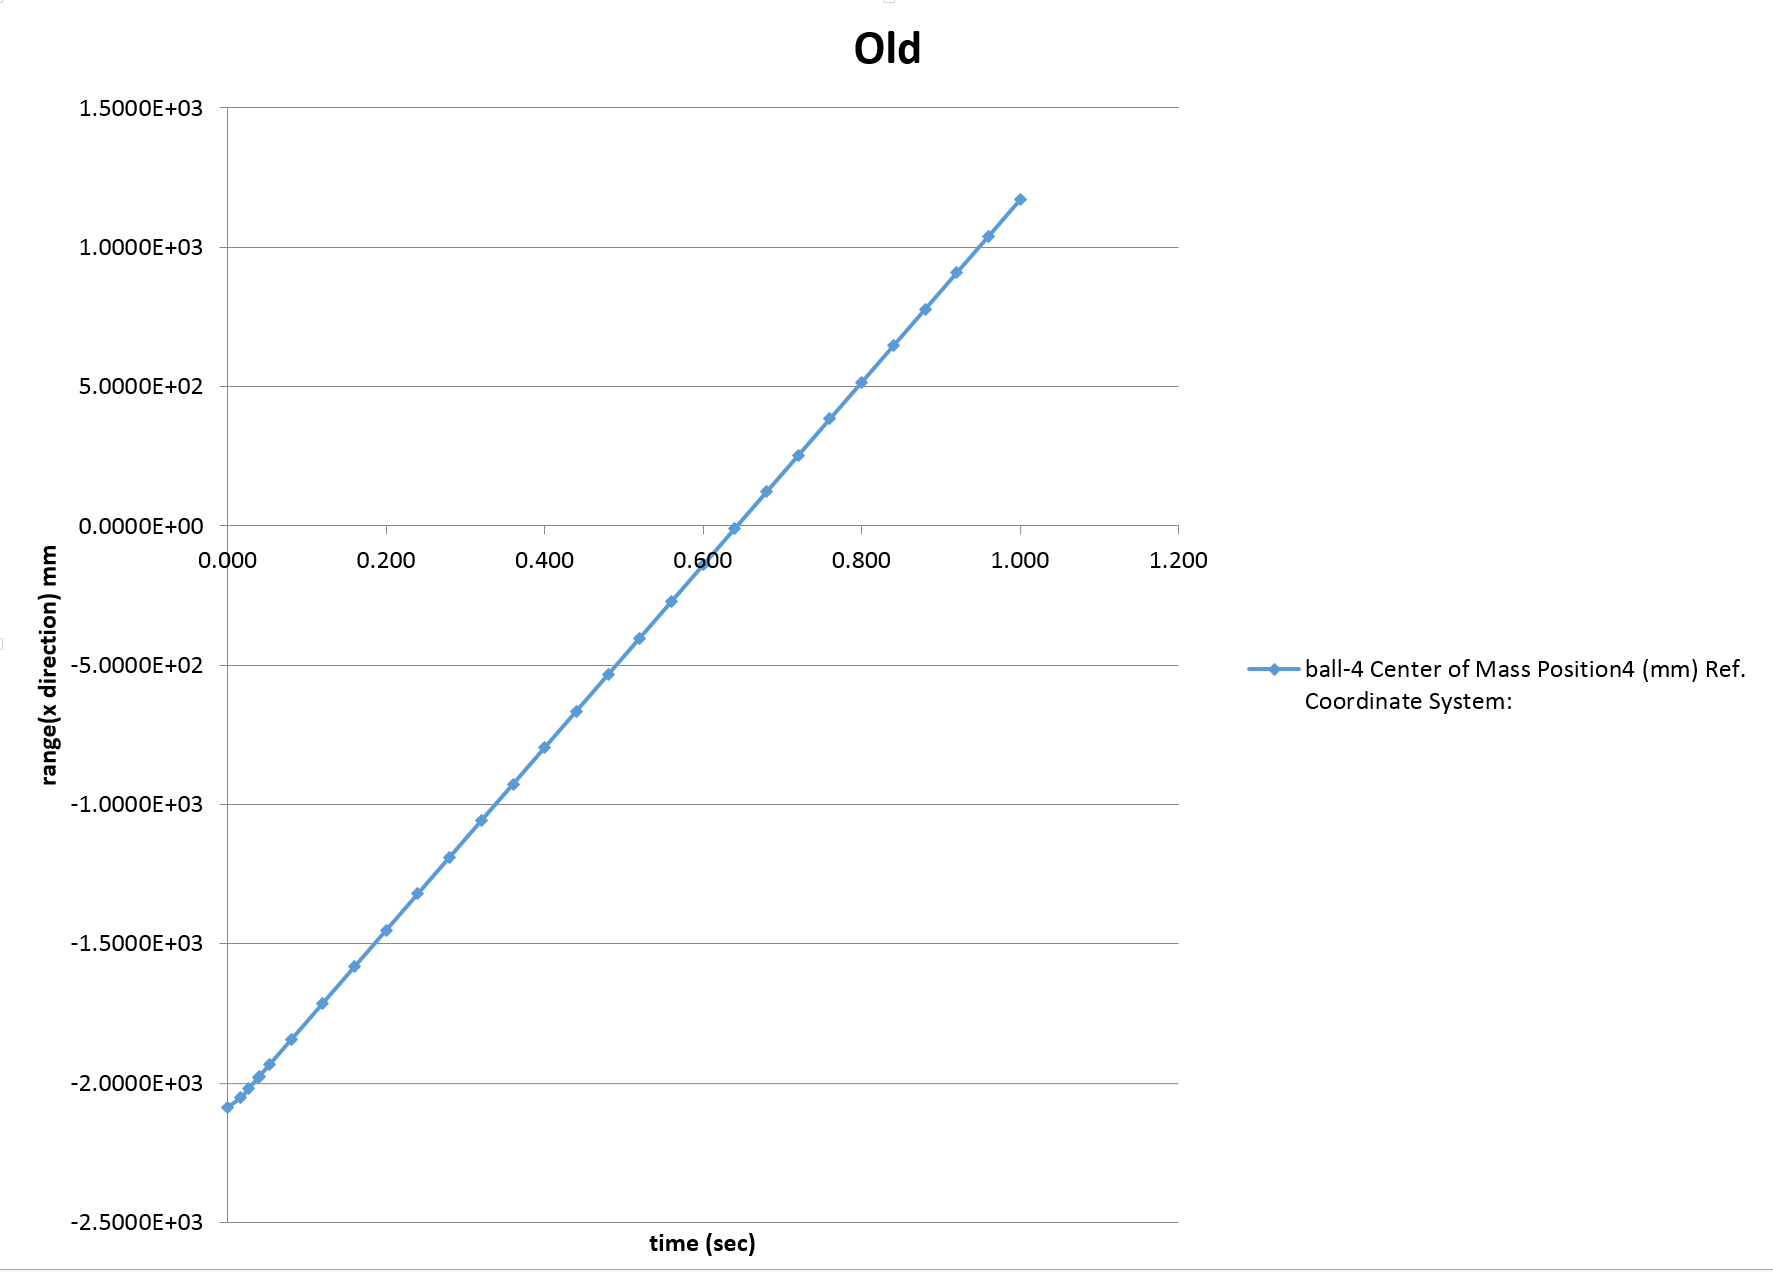
\includegraphics[width=0.8\textwidth]{images/OldBallPlot.png}
%	\caption{Position time graph for a ball being kicked by the old chip kicker}
%	\label{fig:OLDPLOTBALL}
%\end{figure}\\
\\
In conclusion, the new chip kicker can kick the ball further than the old one. The most important point here is that the new chip kickers design made its process of manufacturing much easier and faster. %Also new design of kicking device is in a way that it can be easily disassembled from the robot which makes its repair process much faster. Faster robot repairing means having more robots operate when the match is taking place.




\newpage
\section*{Robot WALL-E Hardware Description [OPL Template]}
\label{sec:annex-OPL}
% In this section briefly describe the software and hardware of the robot

\setlength\intextsep{0pt}
\begin{wrapfigure}[10]{r}{0.3\textwidth}
	\centering
	\includegraphics[width=0.4\textwidth]{images/wall-e.jpg}
	\caption{Robot WALL-E}
	\label{fig:wall-e}
\end{wrapfigure}

Robot WALL-E has the patented \textit{\BnL Optimized Design} for garbage recollection. Specifications are as follows:

\begin{itemize}
	\item Base: \BnL all-terrain base (differential pair), 2.5m/s max speed.
	\item Torso: \BnL compressor with solar charger.
	\item Left and right arms: Mounted on torso. \BnL 7DOF, anthropomorphic. Maximum load: 20kg.
	\item Neck: \BnL telescopic neck with pan and tilt.
	\item Head: 3DOF \BnL Expressive Eyes
	\item Robot dimensions: height: 1.2m (max), width: 0.7m depth 0.8m
	\item Robot weight: 50kg.
\end{itemize}

\noindent\textit{Also our robot incorporates the following devices:}

\begin{itemize}
	\item \BnL Battery charge indicator
	\item \BnL Auto-focus all-purpose cameras
	\item \BnL 7DOF heavy duty fingers
	\item \BnL Cockroach
\end{itemize}

\section*{Robot's Software Description}
% Please describe in this section the software you are using to control your robot. Consider the following example:

\textit{For our robot we are using the following software:}

\begin{itemize}
	\item Platform: \BnL Operating System
	\item Navigation: \BnL Navigator
	\item Face recognition: None. Not designed for human interaction.
	\item Speech recognition: \BnL All-purpose recognizer \cite{bnl1}.
	\item Speech generation: None. Not designed for human interaction.
	\item Object recognition: \BnL Trash Seeker Algorithm (See previous sections).
	\item Arms control and two-hand coordination: \BnL automatic controller \cite{bnl2}.
\end{itemize}

\section*{External Devices}
% Please describe in this section the external devices used by your robot. Consider the following example:

\textit{WALL-E robot relies on the following external hardware:}

\begin{itemize}
	\item \BnL Garbage Compactor
	\item \BnL EVA unit
	\item \BnL Data Cluster
	\item $3 \times$ \BnL Ultra-Power laptops.
\end{itemize}

\section*{Cloud Services}
% Please describe in this section the Cloud Services and online software used by your robot. Consider the following example:

\textit{WALL-E connects the following cloud services:}
\begin{itemize}
	\item Localization and mapping: \BnL Geolocalization system \cite{bnl3}.
\end{itemize}
%\newpage
\section*{M-O Software and External Devices [SSPL Template]}
\label{sec:annex-SSPL}
% In this section briefly describe the software and hardware of the robot

\setlength\intextsep{0pt}
\begin{wrapfigure}[10]{r}{0.3\textwidth}
	\centering
	\includegraphics[width=0.4\textwidth]{images/m-o.png}
	\caption{Robot M-O}
	\label{fig:m-o}
\end{wrapfigure}

We use a standard \textit{Buy'N Large} M-O robot unit. To differntiate our unit, an orange marker has been added on its top.

\section*{Robot's Software Description}
% Please describe in this section the software you are using to control your robot. Consider the following example:

\textit{For our robot we are using the following software:}

\begin{itemize}
	\item Platform: \BnL Operating System
	\item Face recognition: None. Not designed for human interaction.
	\item Speech generation: None. Not designed for human interaction.
	\item Object recognition: \BnL Dirt Detector Algorithm (See previous sections).
	\item Mop unit: \BnL automatic controller \cite{bnl2}.
\end{itemize}

\section*{External Devices}
% Please describe in this section the external devices used by your robot. Consider the following example:

\textit{M-O robot relies on the following external hardware:}

\begin{itemize}
	\item \BnL Mother-ship
	\item \BnL Data Cluster
	\item $3 \times$ \BnL Ultra-Power laptops.
\end{itemize}

\section*{Cloud Services}
% Please describe in this section the Cloud Services and online software used by your robot. Consider the following example:

\textit{M-O connects the following cloud services:}
\begin{itemize}
	\item Localization and mapping: \BnL Geolocalization system \cite{bnl3}.
	\item Navigation: \BnL Navigator
	\item Speech recognition: \BnL All-purpose recognizer \cite{bnl1}.
\end{itemize}

\nocite{*}

%%%%%%%%%%%%%%%%%%%%%%%%%%%%%%%%%%%%%%%%%%%%%%%%%%%%%%%%%%%%%%%%%%%%%%%%%%%%%%%%%%%%
%
% References
%
%%%%%%%%%%%%%%%%%%%%%%%%%%%%%%%%%%%%%%%%%%%%%%%%%%%%%%%%%%%%%%%%%%%%%%%%%%%%%%%%%%%%

\newpage
\bibliographystyle{unsrt}
\bibliography{references}



\end{document}
